\subsubsection{Caso d’uso UC8.2.1.6: Modifica ordinamento di stringhe}
	\label{UC8.2.1.6}
	\begin{figure}[h]
		\centering
		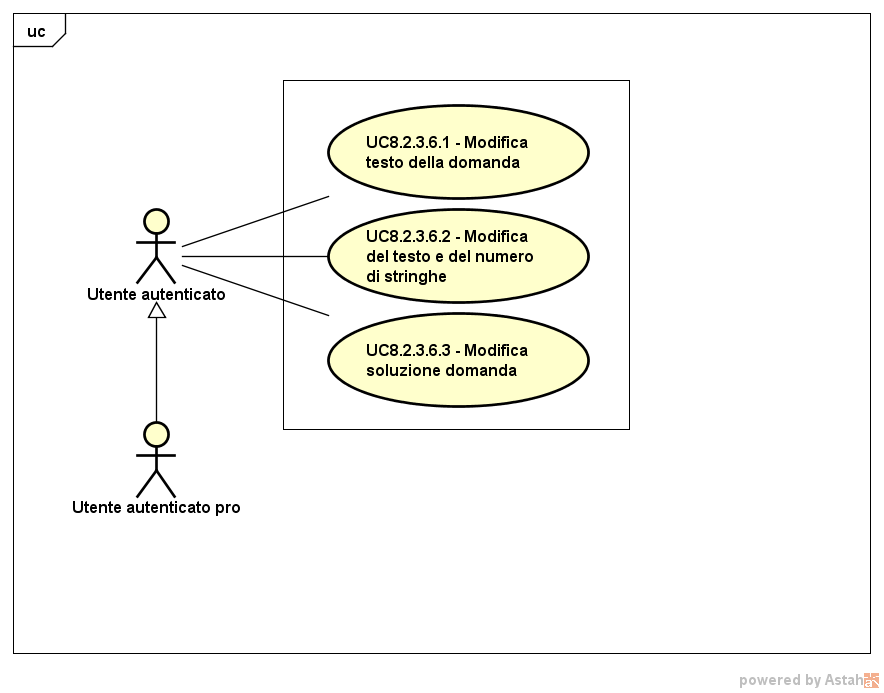
\includegraphics[scale=0.45,keepaspectratio]{UML/UC8_2_3_6.png}
		\caption{UC8.2.1.6: Modifica domanda ordinamento di stringhe}
	\end{figure}
	\FloatBarrier
\begin{itemize}
	\item\textbf{Attori}: utente autenticato, utente autenticato pro;
	\item\textbf{Descrizione}: l'attore può utilizzare la procedura guidata la modifica una domanda a ordinamento di stringhe;
	\item\textbf{Precondizione}: il sistema mostra agli attori il form di modifica dei campi dati per la tipologia di domanda scelta; 
	\item \textbf{Postcondizione}: gli attori hanno modificato la domanda;
	\item\textbf{Scenario principale}:
		\begin{itemize}
			\item Gli attori possono modificare il testo della domanda (UC8.2.1.6.1);
			\item Gli attori possono modificare il testo e il numero delle stringhe che compongono la sequenza della domanda (UC8.2.1.6.2);
			\item Gli attori possono modificare la soluzione della domanda (UC8.2.1.6.3); 
		\end{itemize}
\end{itemize}

\subsubsection{Caso d'uso UC8.2.1.6.1: Modifica testo della domanda}
\begin{itemize}
	\item \textbf{Attori}: utente autenticato, utente autenticato pro;
	\item \textbf{Descrizione}: gli attori possono modificare il testo della domanda;
	\item \textbf{Precondizione}: gli attori hanno selezionato l'opzione di modifica di una domanda;
	\item \textbf{Postcondizione}: gli attori hanno modificato il testo della domanda.
\end{itemize}

\subsubsection{Caso d'uso UC8.2.1.6.2: Modifica del testo e del numero di stringhe}
\begin{itemize}
	\item \textbf{Attori}: utente autenticato, utente autenticato pro;
	\item \textbf{Descrizione}: gli attori possono modificare il testo e il numero di stringhe che compongono la domanda;
	\item \textbf{Precondizione}: gli attori hanno selezionato l'opzione di modifica di una domanda;
	\item \textbf{Postcondizione}: gli attori hanno modificato il testo e il numero delle stringhe che compongono la domanda.
\end{itemize}

\subsubsection{Caso d'uso UC8.2.1.6.3: Modifica soluzione domanda}
\begin{itemize}
	\item \textbf{Attori}: utente autenticato, utente autenticato pro;
	\item \textbf{Descrizione}: gli attori possono modificare la sequenza della soluzione della domanda;
	\item \textbf{Precondizione}: gli autori hanno selezionato l'opzione di modifica di una domanda;
	\item \textbf{Postcondizione}: gli autori hanno modificato la sequenza della soluzione della domanda. 
\end{itemize}